\documentclass[a4paper, 11pt]{article}
\usepackage{CJKutf8}
\usepackage{indentfirst}
\usepackage[dvips]{graphicx}
\usepackage{epsfig}
\usepackage{epstopdf}
\usepackage{graphicx,floatrow}
\graphicspath{{./}{plot/}}

\begin{document}

\begin{CJK*}{UTF8}{gbsn}

\section{问题背景}
最近以``Alpha-Go''为首的人工智能应用层出不求,引起了人们对与Alpha-GO类似的深度学习技术在其他领域相关应用的关注。由于GPU的出现使得大规模计算的实现成为了可能,深度学习在图像处理和自然语言处理方面都有了广泛的应用,但由于对网络的输入输出的格式没有合适的符号来表示,深度学习目前在网络拥塞控制方面并没有大规模应用。当今以移动为中心的异构网络提供各种服务和体验,因此,下一代有线和无线异构网络需要智能化的机制来控制网络流量增长剧烈的趋势。对于传统的神经网络而言,深层神经网络与浅层神经网络的性能往往差不多,它们在计算效率和可扩展性方面有一些缺点以致很难在网络流量方面应用。本文考虑一种包含多个隐藏层的深入学习系统,每个隐藏层计算上一层的非线性变换。首先用贪婪的层次训练方法初始化深度学习系统,然后用反向传播法训练。本篇论文的另一个贡献就是证明,如果设计好输入/输出的traffic pattern,与传统路由方法相比这种方法能更好进行网络拥塞控制。

\section{深度学习建模}
这个神经网络系统的直观表示如图\ref{fig:neural_network}表示。神经网络的输入是路由器的traffic pattern,输出是路由选择线路。由于输入的traffic pattern是连续的,所以每隔时间$\delta$观察一次traffic pattern来将其离散化。输入层有$N$个单元,$N$表示路由器的总个数,用一个$N$维向量表示网络中的traffic pattern,向量中的第$i$个元素表示在时间$\delta$内第$i$个路由器的入站数据包数目。隐藏层对前一层的输入进行非线性的转换,因此神经网络系统可以学到比浅层网络更复杂的结构。输出层继承了隐藏层的非线性变换函数,网络拥塞控制系统的输出是从源节点到目的节点的路由选择通路,用一个二进制的$N$维向量表示,向量中有且只有一个单元值为1,它表示了下一跳的节点。
\begin{figure}[htb]
\centering
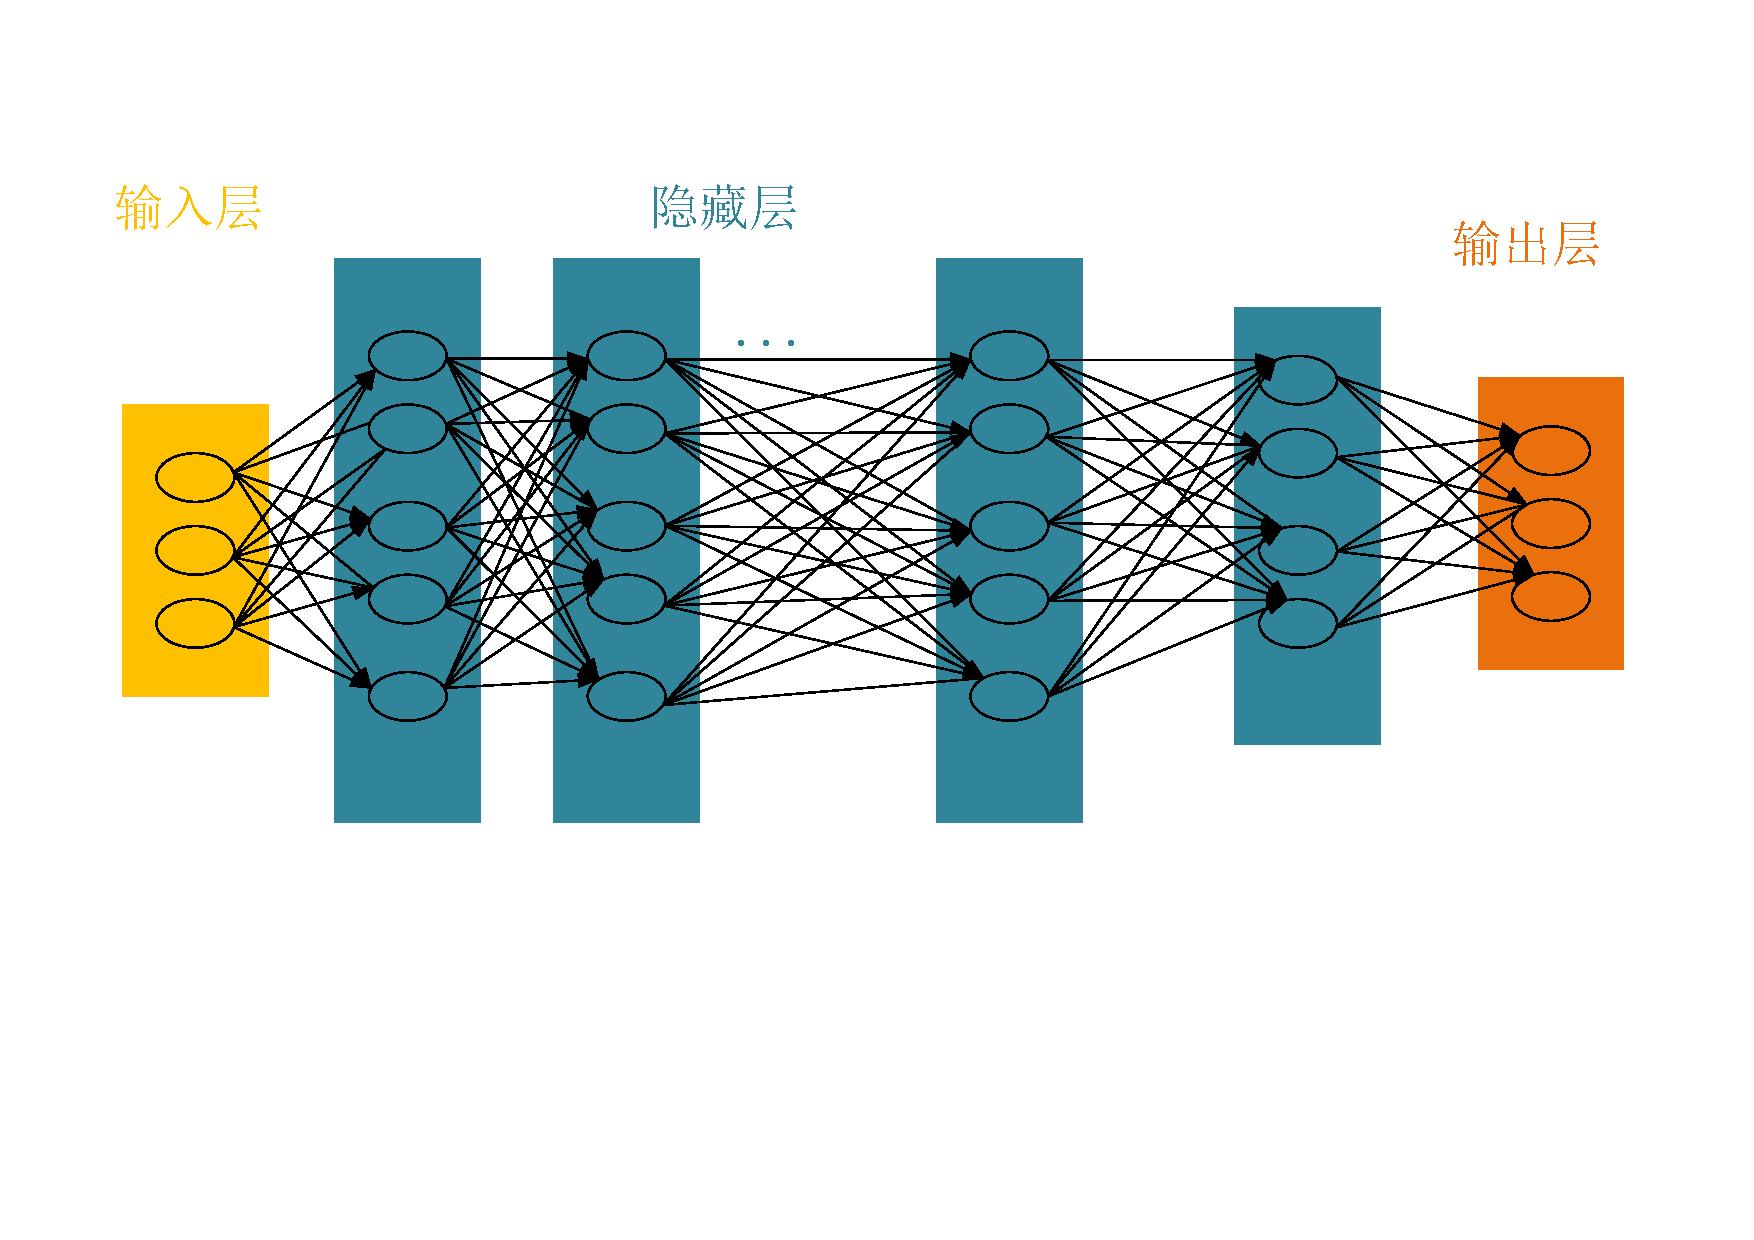
\includegraphics[width=.8\textwidth]{network.pdf}
\caption{深度学习系统模型}\label{fig:neural_network}
\end{figure}
表\ref{table:network_control}表示对这个神经网络系统的性能评估,总共有16个路由节点。第一行表示集中式网络控制方案,这种方案在深度学习系统中有33792个输出单元,计算复杂度非常大。第二行展示了输入向量为$16\times16$的情况,这种数据结构可以提供完整的路由通路,但错误率高达70\%。第三行用非二进制的向量来表示输出的整条路由通路,但误差依旧很大(45\%)。第四行用到上面提到的数据结构,错误率为5\%。最后一行48个输入单元代表了3个$\delta$中的traffic pattern,错误率也是相似的5\%,但是计算复杂度有很高。
\begin{table}[!htb]
\centering
\caption{不同输入和输出结构对网络控制准确率的影响}
\label{table:network_control}
\begin{tabular}{c|c|c|c}
\hline
\textbf{输入节点} & \textbf{输出节点}& \textbf{整条路径或下一跳 } & \textbf{错误率}\\ \hline
16& 33792&整条路径& -\\
16&256&整条路径& 70\% \\
16& 16&下一跳& 45\% \\
16& 16&下一跳& 5\% \\
48& 16&下一跳& 5\% \\ \hline
\end{tabular}
\end{table}

\section{网络控制系统}
我们提出的深度学习系统分为三个部分,初始化,训练和运行。
\subsection{初始化}
初始化的目的是为训练过程提供相关数据。第一种方式是用不同负载和条件下的OSPF路由算法来得到选择的路径,再转换为相应的traffic pattern,另一种方式是在一系列可用数据集中得到相应的拥塞数据。
\subsection{训练}
训练过程的输入和输出分别是$(\hat{x},\hat{y})$,$\hat{x}$表示输入的traffic pattern而$\hat{y}$表示输出的下一跳节点。$\hat{x}$与$\hat{y}$都表示$N$维向量,$N$表示网络中路由器的总数目。$I$表示内部路由(非边缘路由)的数目,训练过程的输出为权重矩阵(Weight Matrix)。
对于每一个边缘路由器,由于它有$N-I-1$个目标边缘路由器所以它需要训练$N-I-1$个深度学习系统,而对内部路由器而言则需要训练$N-I$个深度学习系统。用$DL_{ij}$表示从路由器$i$到节点$j$的深度学习系统,用$WM_{ij}$表示$DL_{ij}$的权重矩阵,训练过程分为两个部分:
\begin{itemize}
  \item 用逐层贪婪训练法(Greedy Layer-wise Training Method)来初始化深度学习系统。
  \item 用反向传播算法来微调深度学习系统。
\end{itemize}

\subsection{运行}
运行的过程简而言之,就是输入原路由的traffic pattern(TP),通过训练得到的$DL$和$WM$来取得下一跳节点,直到下一跳节点是目标节点。
\begin{figure}[htb]
\centering
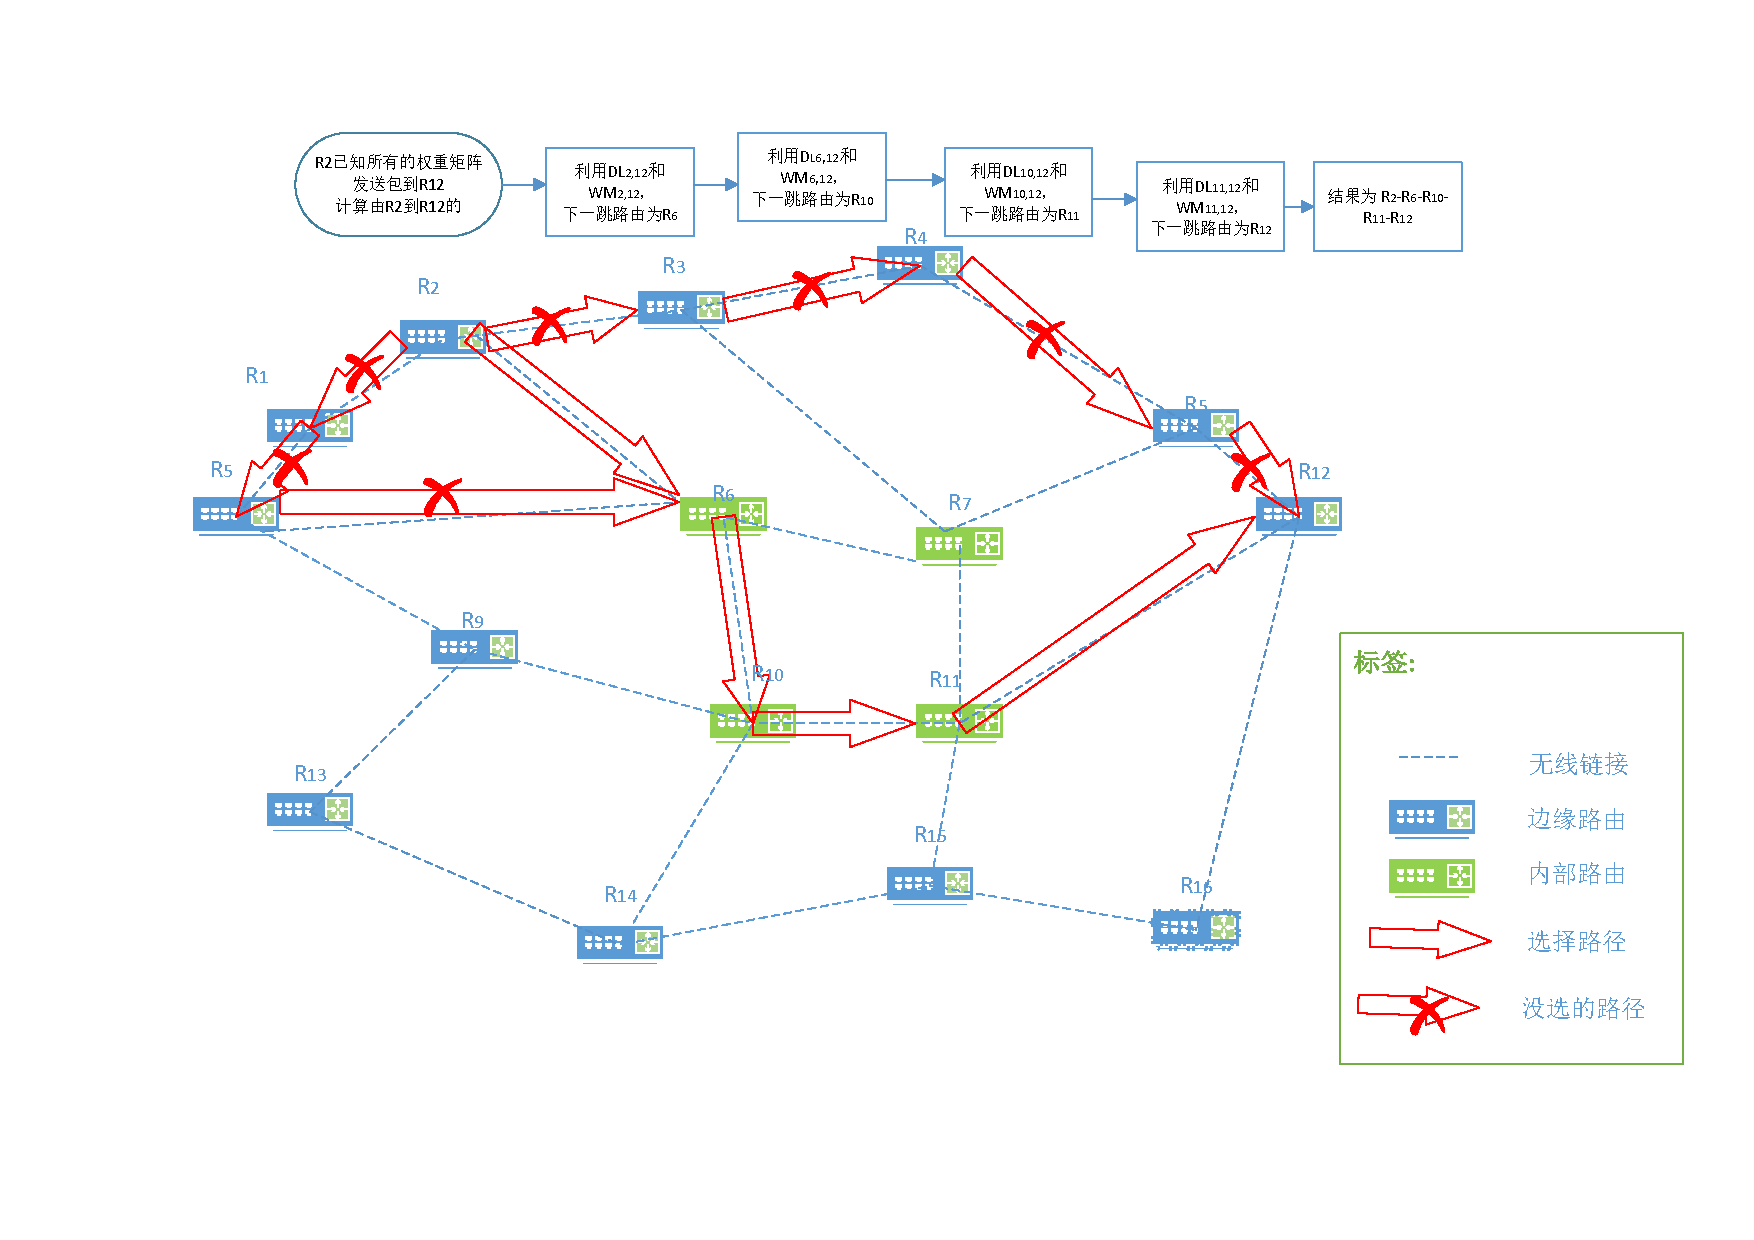
\includegraphics[width=\textwidth]{routing_algorithm.pdf}
\caption{由路由$R_2$发包到$R_{12}$的例子}\label{fig:routing_algorithm}
\end{figure}
图\ref{fig:routing_algorithm}提供了一个简单的例子,$R_k$表示第$k$个路由器。源路由为$R_2$而目标节点为$R_{12}$。在给出了输入模式$\hat{x}$之后,$R_2$需要通过$DL_{2,12}$计算出下一节点,为$R_6$。之后$R_6$通过$DL_{6,12}$计算出下一节点$R_{10}$。$R_{10}$通过$DL_{10,12}$计算出下一节点$R_{11}$,最后可以确定整条路径为$R_{2}\rightarrow R_{6}\rightarrow R_{10} \rightarrow R_{11}\rightarrow R_{12}$。

这种基于时间间隙(time-slot)的同步方法与传统路由策略(OSPF)在固定时间间隙(fixed time intervals)执行类似。但是在运行阶段(running phase)不需要同步。

\section{性能评测}
仿真实验基于C++/WILL API\cite{WILL}。仿真的环境为Intel Core i7 3.60 GHz 以及16GB的RAM。由于仿真实验是运行在一台计算机上,所以设计了一个有16个路由器的中等规模的网络拓扑结构。数据包和控制包的大小为1Kb,链路带宽为8Mb/s,整个网络的数据包生成速率为16.32Mb/s,$\delta$设为0.25s。\cite{Kato2017:MWC}首先研究神经网络不同参数对实验结果的影响,然后就信令开销,吞吐量和时延三个方面来将深度学习系统与传统的OSPF算法进行对比。

神经网络的loss function选取最小均方误差(MSE), 隐藏层的层数选择$\left \{ 4,5,6 \right \}$三种而每一个隐藏层的单元有$\left \{14,16,18,20 \right \}$四种选择,总共评估了12种结构。\cite{Kato2017:MWC}中的结果中得出,4层网络得到的结果最好,因为层数太多可能会发生过拟合(Over-fitting)。当隐藏层单元数为16或者18时均方误差最小,由于隐藏单元数越多计算复杂度越大,所以我们最后选择隐藏层有16个单元的结构。

\textbf{深度学习系统的信令开销远小于OSPF。}这是由于传统的OSPF方法中所有的路由器都需要频繁更新邻居路由的信息,而深度学习的方法中只有边缘路由之间需要交换traffic pattern。

\textbf{深度学习系统的吞吐量大于OSPF。}这是由于深度学习系统可以更快的选择路由路径,所以避免了拥塞和丢包。

\textbf{深度学习的时延远小于OSPF。} 这是由于深度学习能更好的选择合适的路由。

\section{总结}

本文把深度学习的方法应用到了网络拥塞控制中。这个深度学习系统的输入是traffic pattern,输出是下一个节点。通过监督学习能使整个深度学习系统能够尽快找到从一个节点到下一个节点的路径,这种方法在吞吐量,时延和信令开销上的性能比OSPF高很多。

这种方法的\textbf{优点}在于:比较有创新性,将深度学习的方法应用到了流量过程,并且取得了比传统方法更好的性能。

这种方法的\textbf{不足}之处在于:需要大量的数据集来训练数据(supervised learning),收集数据的开销很大。由于网络的性能可能随时间变化较快,所以整个系统有时效性,需要频繁训练。

\end{CJK*}

\vspace{0.5cm} % A white space


\vspace{0.5cm}

\noindent
\bibliographystyle{plain}
\bibliography{internet-te}
%\begin{thebibliography}{}
%
% and use \bibitem to create references. Consult the Instructions
% for authors for reference list style.
%

% Format for Journal Reference
%Author, Article title, Journal, Volume, page numbers (year)
% Format for books
%\bibitem{RefB}
%Author, Book title, page numbers. Publisher, place (year)
% etc
%\end{thebibliography}


\end{document} 